\documentclass[../Document.tex]{subfiles}
\graphicspath{{\subfix{../images/}}}

\begin{document}


\Chapter{COMBINING \acrshort{cp} WITH \acrshort{nlp} TO IMPROVE GENERATION}
\label{chap:gpt+cp}
This chapter details how we combine our previous \cp with a chosen \gls{llm} to try and improve the realism of our generated molecules. By combining a model trained on real drug-like molecules and our \cp model, we believe it is possible to get molecules that are informed by what is in current use while still maintaining the guaranteed validity and property targeting.

The first section will present the combined architecture before going in depth on each part. We will then go over the experiments we did and their results in the next two sections.

The work in this chapter was published as part of a joint article presented at IJCAI25~\cite{ijcai:saikali}.

\section{Architecture}
To combine the two models, we use a combination at inference time (\ie during generation). Our \gls{cpbp} model takes the \gls{llm}'s prediction probabilities over the next token as an input and updates them using \bp. The combined model then samples the next token from this new distribution and sends this new string as an input to the \gls{llm}.

This combined model, called \gls{geai-blanc}, can be seen in Figure~\ref{fig:combined-architecture}. We start with the start token and, after each iteration, sample a new token that is informed by both the \gls{llm} and our \gls{cpbp} model.

\begin{figure}
    \centering
    \input{figures/fig:combined-architecture}
    \caption[Combined \cp and token-by-token generator architecture.]{Combined \cp and token-by-token generator architecture. In our case, the token-by-token generator is a \gls{llm}, but any other can be used as long as it was trained on \smiles strings. The \nn outputs a probability distribution over the next token, $X_t$ in our example. This distribution is given as the outside belief of the \oracle constraint. After a few iterations of \bp, we get our new distribution and sample for the next token. This process starts by inputting the start token to the \nn.}
    \label{fig:combined-architecture}
\end{figure}

\subsection{\gls{llm}}
We chose to use the \gls{gpt} model, GPT2-ZINC480M-87M\footnote{\url{https://huggingface.co/entropy/gpt2_zinc_87m}} (henceforth referred to simply as GPT).
It has 87M parameters and was trined on 480M molecules from the ZINC database\footnote{\url{https://zinc.docking.org/}}.
This is the same database that we have partial access to (we can access 250k molecules).
It is a transformer model trained to generate molecules in the standard string representation \smiles (Fig.~\ref{fig:combined-model-molecule} gives an example).

\begin{figure}[t]
    \centering
    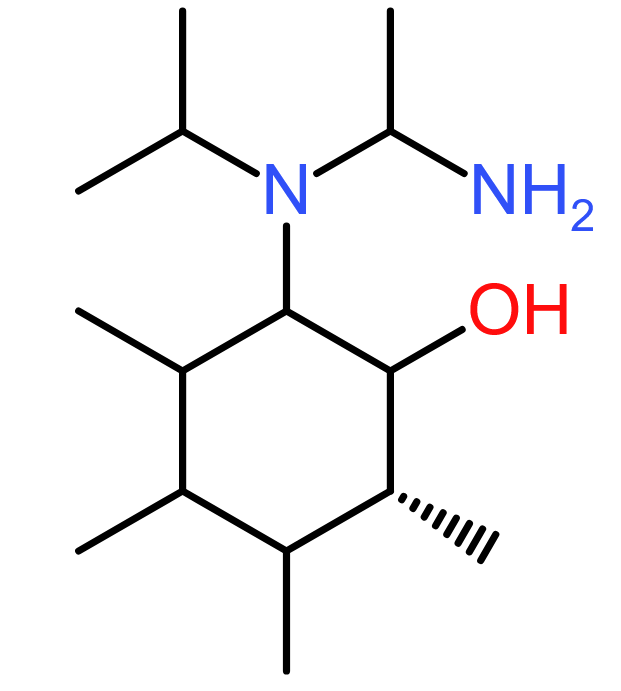
\includegraphics[width=0.25\columnwidth]
    {images/example_molecule.png}
    \caption{``C[C@H]1C(O)C(N(C(N)C)C(C)C)C(C)C(C)C1(C)", a molecule of weight  256.3 Da and PPL=1.8487
    generated by GeAI-BLAnC.} % poids approximatif de 254 Da
    \label{fig:combined-model-molecule}
\end{figure}

The use of a token-by-token generation model allows us to change the probability distribution over the next token before sampling and is necessary for this combined architecture to work.

However, changing this distribution might overpower the \gls{llm}'s message with the \gls{cpbp} model's message. This will be studied later in our experiments through the use of the perplexity metric (which will be explained in Section~\ref{sec:gptcp-experiments}).


\subsection{Oracle Constraint}
\label{sec:oracle-constraint}
The \oracle constraint is a unary constraint defined as follows: \oracle($X,p$). $X$ is a finite-domain variable and $p$ is a fixed probability mass function over the domain of $X$.
In our case the variable is $X_t$, representing the token at step $t$ and $p$ is the \nn's probabilities for the current token $x_t$.
Uncharacteristically, this constraint does not enforce a relation but only associates a probability to each domain value.
Its sole purpose is to contribute messages to variable $X_t$ during \bp in the same way as the other constraints in the \cp model.
Without the \oracle constraint, the resulting marginals would only take into account the satisfaction of $C(X_1,\ldots,X_n)$ (\ie the satisfaction of the constraints over the variables) and not what was learned from the dataset.
Therefore, the \oracle constraint is our way of integrating the \nn's knowledge into the process of \cpbp.

To balance this integration, we can associate a weight to our constraints, in this case we would adjust the weight of the \oracle constraint (as will be shown later in our experiments).
This weight affects the marginals sent by constraints during \bp (and not the filtering nor the hardness of the constraint).
Given a positive weight $w$ (the default value being 1) each marginal $p_X(v)$ for a value $v$ in the domain of variable $X$ is raised to the power of that weight and normalized, yielding new marginal $(p_X(v))^w / \sum_{d \in D(X)} (p_X(d))^w$.
As a result, a weight $w>1$ accentuates the disparities between marginals
while $0 < w < 1$ lessens them and makes them more uniform.
We will use such a weight on the \oracle constraint in order to control its importance on the resulting distribution.


\subsection{Communication}
\label{sec:cpgpt/communication}
Since the two models are in different programming languages, \gls{gpt} is in Python while MiniCPBP (the solver from Section~\ref{sec:valid-experiments}) is in Java, we had to set up a way for them to communicate.
We could do this by integrating one model into the other language, however we chose to use a minimalistic \gls{http} server approach.

By making the \gls{gpt} model a server with its own interface, we can easily change the model being used, and we can allocate more resources to it if needed.
The \gls{gpt} model can compute the next token's probability distribution fast enough that it can keep up with multiple client instances making requests.

The client instances in question are the \gls{cpbp} model. It makes an asynchronous \gls{http} request to the server with the current molecule in the request. The server decodes the molecule and calculates the next token's probabilities.

An issue we encountered is that our \gls{cpbp} model's language is made up of relevant single tokens in the \smiles alphabet.
However, the \gls{gpt} model's language is made up of n-grams, which includes single tokens, but also includes n-grams made up of multiple tokens.
If we were to return those probabilities as they are, our client instance would be unable to input them into the \oracle constraint.
We first convert the result into something our client can understand.

To do this, we pass over every n-gram and associate its probability to the first token that appears in it.
If the first token already has an associated weight, we sum the two probabilities into a new one.
Since we get the probability of every n-gram in the \gls{gpt} model, every token from our \gls{cpbp} model's language is guaranteed to have an associated probability, though that weight may be $0$ if every n-gram the token leads has a null-probability.
This conversion also allows us to remove any unwanted tokens that our \gls{cpbp} model does not support (\eg higher cycle number tokens).
Finally, during this process, we also change the end-of-sequence token, ``</s>'', to our padding token, ``\_'', since they functionally represent the same thing. Once we place a padding token, the only thing that can follow are more padding tokens. 

With this, we have a functioning \gls{http} server that takes the current molecule as input and returns the probability distribution over the next token's value in our \gls{cpbp} model's language.


\section{Experiments}
\label{sec:gptcp-experiments}
This section will detail the experimental context and any steps required to reproduce our results.

With our experiments, we wish to show two things.
First, we want to further our findings from Section~\ref{sec:valid-experiments} and evaluate the advantages of \bp when looking for a solution as per our third research question.
We also aim to show that our approach more consistently generates sequences exhibiting the desired structure while still reflecting what the \nn has learned from the training corpus.

\paragraph{\gls{gpt} model's settings.}
As mentioned prior, we use the GPT2-ZINC480M-87M\footnote{\url{https://huggingface.co/entropy/gpt2_zinc_87m}} model that was trained on 480M molecules from the ZINC dataset. 

During generation, we kept the model's default configuration with the following exceptions:
we limited the generation to one new token at a time as per Fig.~\ref{fig:combined-architecture}, 
we set the model's temperature to $1.5$ which gives more varied results as reported by the model's authors, 
we decreased the maximum length of the molecule to fit our target length, 
and we disabled the early stopping parameter.

\paragraph{Changes to the \cp solver.}
During most of our tests, we choose to disable the backtracking ability of our \cp solver, MiniCPBP\footnote{\url{https://github.com/PesantGilles/MiniCPBP}}.
We do this to allow a more faithful comparison between the models.
We keep one test with the backtracking active to evaluate the differences.

We will detail which search heuristics were used during generation later on.

\paragraph{Experimental conditions.}
We attempt to generate 100 molecules.
Our experiments were run using an 8-core processor with a core speed of 4.20 GHz and 64GB of \gls{ram}.
All our code and data for these tests are available\footnote{https://github.com/cravethedave/MiniCPBP/tree/ijcai-2025}.
As an initial input to the \gls{gpt} model, we use the start-of-sequence token, ``<s>''.

\subsection{Chosen constraints}
For these tests, we did not use all the constraints described previously in our \cp model.
We only need a subset of the constraints for the goals set earlier.

All constraints relating to the validity of the \smiles string are necessary to ensure that any generated final result respects \smiles notation. These are the constraints described in Section~\ref{sec:validity-constraint-definition}.

We do not keep any of the structural constraints described in Section~\ref{sec:structural-constraints-definition}. While they would add complexity to the problem, they do not require long-term structure the way the property constraints do.

While all property constraints from Section~\ref{sec:property-constraints-definition} introduce some form of long-term structure to the molecule, only one is required to evaluate it. We chose the molecular weight constraint for three reasons: most tokens in the chain will have an effect on the weight, the \gls{gpt} model was not trained on this property, and it is more accurate than the \emph{logP} constraint.

Overall, we apply the following constraints. Note that the targeted molecular weight is now between 200 and 275 Daltons.
This weight is only achieved by 20.48\% of the 40-token molecules observed in the datasets.
% >>> len(correct_weight)/len(correct_size)
% 0.20484601212374826
% >>> len(correct_weight)/len(molecules)
% 0.16120255193771363

\begin{align*}
    &\text{Validity Constraints:}\\
    &\hspace{16pt} \texttt{grammar}(\langle X_1, X_2, \ldots, X_{40} \rangle, \mathcal{G}_{\texttt{SMILES}})\\
    &\hspace{16pt} \among(\langle X_1, X_2, \ldots, X_{40} \rangle, \{j\}, \{0,2\})\ \forall\ j\ \vert\ 1 \leq j \leq 6\\
    &\hspace{16pt} \regular(\langle X_1, X_2, \ldots, X_n \rangle, \mathcal{A})\\
    &\text{Molecular Weight Constraint:} & &\\
    &\hspace{16pt} \element({\cal T}^w, X_i, W_i)\ \forall\ i\ \vert\ 1 \leq i \leq n\\
    &\hspace{16pt} \somme(\langle W_1, W_2,\ldots,W_n \rangle, S^w)\\
    &\hspace{16pt} 200 \leq S^w \leq 275
\end{align*}


\subsection{Evaluation metrics}
To evaluate our different models, we use three metrics: time, success rate and perplexity.

The time is self-explanatory, we measure the average time to generate a molecule over all successful molecules generated. This means that unsuccessful runs aren't accounted for in this average. We also set a time limit on the \gls{cpbp} model running with backtracking in case the search takes too long. The time limit was set to 10 minutes.

As for the success rate, it is evaluated as the number of successfully generated molecules out of the 100 attempts. However, we categorize a molecule as "successfully generated" if the generated molecule is valid and respects all constraints that we defined.

Finally, perplexity~\cite{perplexity} is a common metric in NLP:
$$
    \mbox{PPL}(x_1,\ldots,x_n) = \exp \left( - \frac{1}{n} \sum_{t=1}^n \log  p(x_t | x_1,\ldots,x_{t-1}) \right)
$$
The higher the perplexity, the less likely it would be generated by the neural model and the more surprising it is with respect to the training set.
This is particularly interesting for our \cp model as it may disagree with the probability distribution it receives from \gls{gpt} and modify it. This could increase the perplexity score for the current token if the chosen value is one that \gls{gpt} would be less likely to choose.
We also consider perplexity for individual tokens, $1/p(x_t | x_1,\ldots,x_{t-1})$, in order to track its behavior across the whole sequence.


\subsection{Tested model combinations}

\subsubsection{CPBP with backtrack}
This is the default solving method for our \gls{cpbp} solver.
It should have the highest success rate as it can backtrack to fix its mistakes while the other methods will be limited to token-by-token generation.
Its perplexity score could be high, but it'll be interesting to see if it differs from the \cp model with no backtracking.

To ensure the results are as close to the other models, allowing for a better comparison, we use a lexicographic variable choice (\ie in order from left to right) and a biased wheel selection for the value (\ie weighted random or roulette wheel selection) according to the marginal distribution.

All further models will generate the sequence token-by-token.

\subsubsection{CPBP no backtrack}
By removing the backtracking from our model, it may end up making mistakes.
However, this serves as a better comparison to the \gls{gpt} models as we cannot backtrack to fix our mistakes, which is how the \cp model will be used in the combined architecture.

\subsubsection{GPT}
The first \gls{gpt} model is run without any input from the \cp side of things.
This serves as our baseline for the perplexity score.
Once we add \cp to the setup, we'll be able to see how it affects the success rate of our model.

\subsubsection{GPT + CP}
By adding the \cp component to our \gls{gpt} model, we expect the success rate to rise in exchange for an increase in perplexity.
This model does not use \bp and thus the integration between the two models is slightly altered.
Instead of modifying the \gls{gpt} model's probabilities, we simply use \cp to eliminate values that would breach one of our constraints and then normalize the probabilities of the possible values that are left.
We then proceed normally, using a biased wheel selection.

\subsubsection{GPT + CPBP}
Finally, this model is the one presented in Figure~\ref{fig:combined-architecture}.
It utilizes \bp to modify the probabilities received by the \gls{gpt} while also getting rid of values breaching contraints.

As mentioned in Section~\ref{sec:oracle-constraint}, we can modify the weight of the \oracle constraint to increase or decrease its influence on the generated sequence.
We test this model using a baseline constraint weight of 1, as well as 0.5 and 1.5 to observe the effects it has on the perplexity and the success rate. The time should not be affected by this change.


\section{Results}
This section will go over the results presented in Table~\ref{tab:gptcp-results} for the different model combinations that we described previously.

\begin{table}[t]
    \centering
    \begin{tabular}{l r r r}
        \hline
        method & success(\%)$\uparrow$ & PPL$\downarrow$ & time(s)$\downarrow$\\
        \hline
        % \midrule
        %GPT one-shot            & 5 & 3.09 & 0.0004 mins \\
        CPBP (backtrack)        & 100   & 1236.71   & 125.4 \\
        CPBP (no backtrack)     & 59    & 503.48    & 62.4 \\
        GPT                     & 7     & 5.30      & 1.2 \\
        GPT+CP                  & 18    & 13.50     & 25.2 \\
        GPT+CPBP ($w=1$)        & 92    & 8.35      & 67.2 \\
        %\midrule
        GPT+CPBP $w=0.5$        & 82    & 17.30     & 70.8 \\
        GPT+CPBP $w=1.5$        & 72    & 8.14      & 63.6 \\
        \hline
    \end{tabular}
    \caption[Success rate, average perplexity, and average runtime over 100 attempts to generate weight-constrained 40-token molecules.]{Success rate, average perplexity, and average runtime over 100 attempts to generate weight-constrained 40-token molecules. The arrows near the column heads indicate what the goal is for this column (\ie minimize or maximize).}
    \label{tab:gptcp-results}
\end{table}

\paragraph{\gls{cpbp} with and without backtrack.}
As we expected, the backtracking model has the highest success rate at the cost of having a very high perplexity and run time. It takes twice as long to solve when we use backtracking, but we achieve a perfect success rate.
The success rate of the no-backtracking model is much lower than we anticipated. By eliminating values that lead to unsolvable sequences, we thought the model would still perform with very few errors. However, \bp is a heuristic, and we are using a biased wheel selection, meaning we might make multiple non-ideal choices which lead to an unsolvable sequence.

What's interesting to note is that backtracking seems to increase the perplexity. We believe this is due to a type of ``survivor bias''. When we have backtracking enabled, a non-ideal decision, which would have lead to an unsolvable sequence in the no-backtrack model, can still be solved using backtracking and results in a molecule that is atypical and has a high perplexity score. In other words, the perplexity is higher because molecules that have a high perplexity are harder to solve and end in failure when we don't have backtracking.

\paragraph{\gls{gpt} model alone.}
Contrary to the previous two models, this one's success rate is the lowest, but it also achieves the best perplexity score in the least time.
Since the model is used to calculate perplexity, it holds that molecules generated purely with this model would have the lowest score.

A reminder that a successful molecule is one that respects validity \emph{and} the molecular weight. The model generates more valid molecules, but as it was not trained to target the specified molecular weight range, it does not perform well in terms of success.

\paragraph{\gls{gpt} with an added layer of \cp.}
Just by adding a layer of \cp at inference time, we double our success rate.
Unfortunately, as we do a biased wheel selection using the \gls{gpt} model's probabilities, we still end up making mistakes.
This model's increased success rate does show that \cp filters out some wrong choices, however there is a significant increase in both time and perplexity.

\paragraph{\gls{gpt} + \gls{cpbp}, the full combined architecture.}
This model is the final one we proposed, a combined architecture that utilizes both the learned information from a \gls{gpt} model and the \bp of our \cp model.

We ran tests with three different \oracle constraint weights: 0.5, 1 and 1.5.
The success rate of the baseline model (weight of 1) is the highest of the three. 
As was expected, by increasing the weight of the constraint, we decrease the perplexity as we are giving more weight to the \gls{gpt} model's message (and inversely when we decrease the weight of the constraint).
However, what was unexpected is the decrease in success rate regardless of which way we shift the weight.
Intuitively, one would expect the success rate to increase as we decrease the \oracle constraint's weight, giving priority to the hard constraints.
But, as we can see, the \gls{gpt} model contributes to the validity of the model and decreasing the strength of its message leads to more mistakes.
There might be another point between 0.5 and 1.5 with a higher success rate, but finding it falls outside the scope our work.
When we decrease the constraint's weight, we see a clear increase in perplexity: giving more weight to the constraint model over the \gls{gpt} model would have that effect.

Overall, this final model performs incredibly well in terms of success rate, firmly beating \gls{gpt} and \gls{cpbp} without backtracking.
It takes more time, roughly one minute per molecule, far more than \gls{gpt}. We can see that a large part of that time comes from the added \bp calculations (note the difference between \gls{gpt}+\cp and \gls{gpt}+\gls{cpbp}). We will discuss ways to mitigate this in our future work.
The perplexity score stays pretty low even after adding the \gls{cpbp} component, far lower than \gls{cpbp} on its own and not too far above the \gls{gpt} model alone. 

Something very interesting is how the addition of \bp lowers the perplexity.
We expected the opposite to happen, where adding \bp would change the \gls{gpt} model's probabilities during sampling and lead to a higher perplexity.
This could be explained by high-cost decisions the no \bp model has to make.
Since \bp guides the search towards probable solutions, we believe the no \bp model ends up in bottlenecks where it has to make multiple high-cost decisions to maintain solvability. Meanwhile, the \bp model anticipates these problems and guides the search towards a more likely solution, making fewer high-cost decisions earlier to avoid multiple high-cost ones later.
This can be seen in Figure~\ref{fig:molecule-heatmap}, where the model with no \bp starts off with very low perplexity choices and slowly gets worse. Meanwhile, the \bp variants make a high-cost decision early, allowing future decisions to remain low.

\begin{figure}[h]
    \centering
    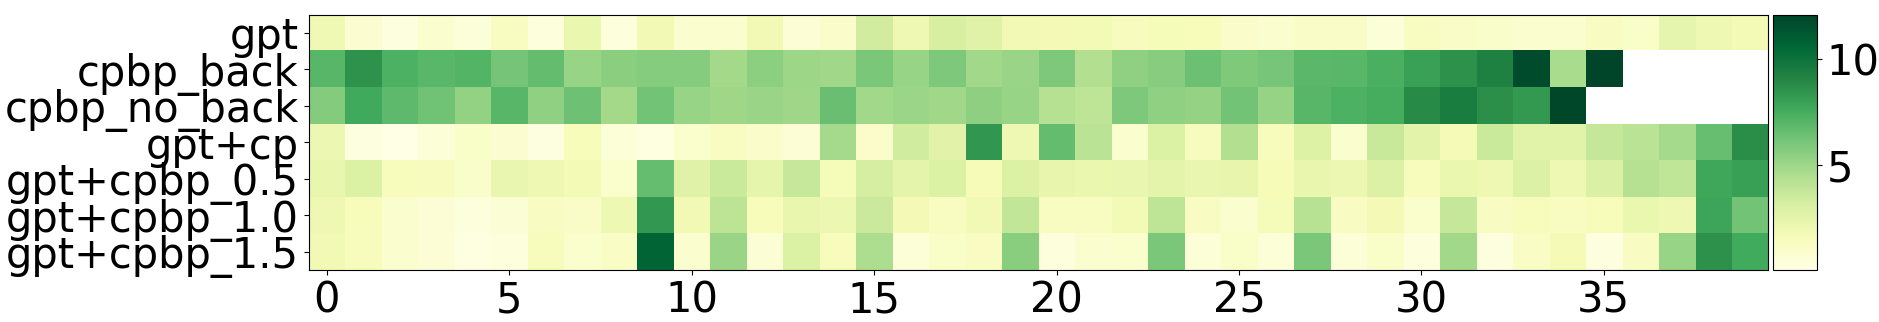
\includegraphics[width=1.0\linewidth]{images/heatmaps.png}
    \caption[Average perplexity indexed by token (darker is higher).]{Average perplexity indexed by token (darker is higher).}
    \label{fig:molecule-heatmap}
\end{figure}

The combined architecture successfully targets the molecular weight desired, even though the base \gls{gpt} model was not trained to do so, while still maintaining a low perplexity.
Admittedly, the time is high, but we believe this can be improved and does not prevent an answer to our fourth research question: How can we combine a \acrshort{cp} model with a \acrshort{nlp} model to improve the realism of generated sequences and is it an effective method?
We have shown how to combine the two models with the help of the \oracle constraint and the results indicate that it is effective at targeting the specified constraints without overpowering the information learned by the \gls{gpt} model.



\end{document}